% Figura 4 - choropleth do deserto de fluxo (F1). src: 12_fig_desert_maps.py
\begin{figure}[t]
\centering
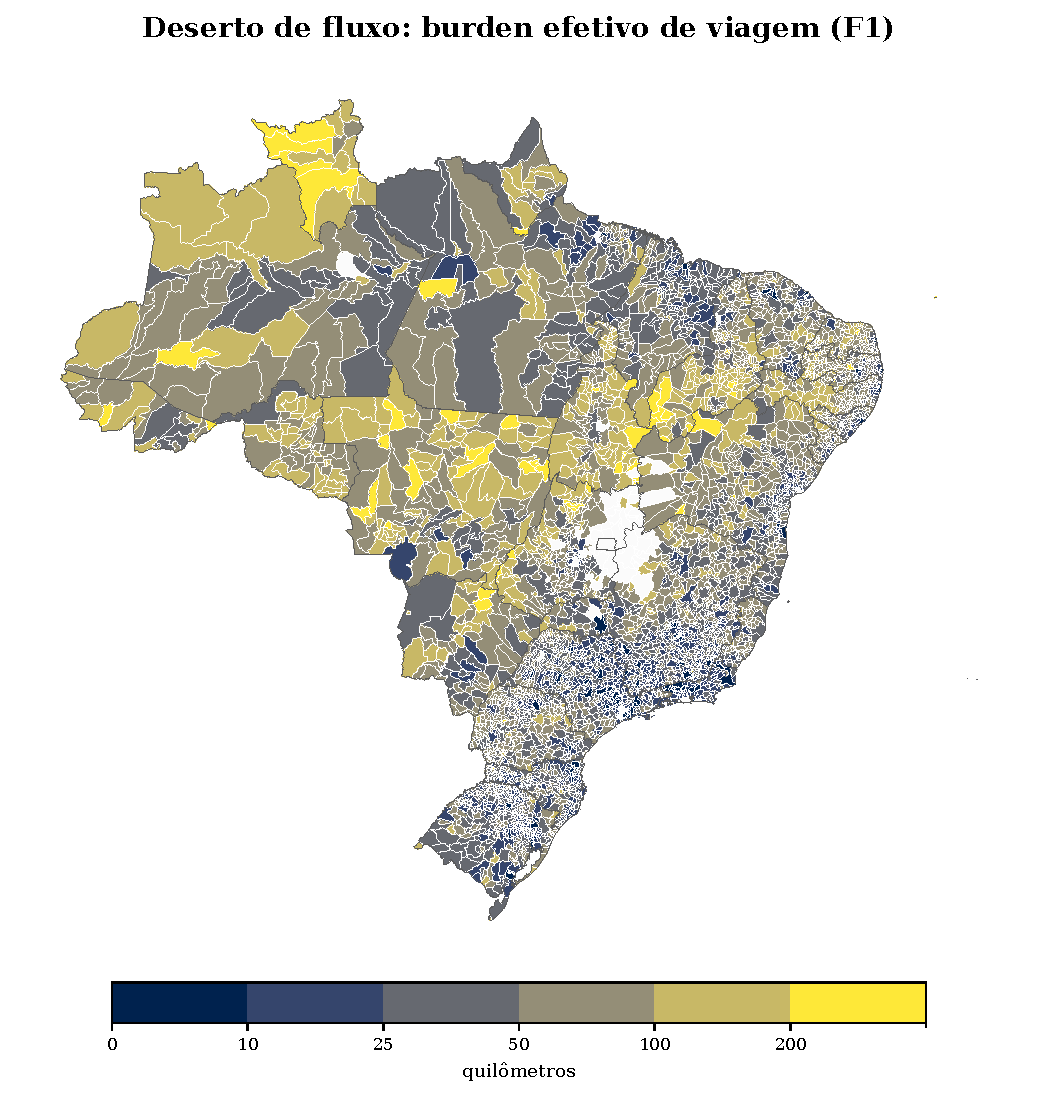
\includegraphics[width=0.86\linewidth]{../04_figures/fig4_flow_map.pdf}
\caption{\textbf{Deserto de fluxo: burden efetivo de viagem (F1).} Cada município
colorido pelo burden efetivo de fluxo --- distância de viagem ponderada por onde
os pacientes de fato internam ---, 2015--2022, na mesma escala de quilômetros da
Figura~\ref{fig:distance_map}. O mapa é visivelmente mais quente: o burden
efetivo mediano (\valMedFround~km) é o triplo da distância mediana ao hospital mais próximo,
e o interior do Nordeste, do Centro-Oeste e do Norte carrega burden alto onde a
distância sugeria proximidade. Projeção Brasil Polyconic (EPSG:5880). Fonte:
SIH/DATASUS, OSRM, IBGE.}
\label{fig:flow_map}
\end{figure}
